\documentclass[draft]{article}
\usepackage[a4paper]{geometry} %use this if you want wider text
\usepackage[utf8]{inputenc}

\newcommand{\dfrac}[2]{\frac{d #1}{d #2}}
\usepackage{tikz}
\usetikzlibrary{intersections}
\usetikzlibrary{quotes,angles,positioning}
\usetikzlibrary{arrows,decorations.pathmorphing,backgrounds,positioning,fit,petri}

\title{TikZ}
\author{Pontus Vikstål}
\date{April 2019}


\begin{document}

\maketitle
%%%%%%%%%%%%%%%%%%%%%%%%%%%%%
%                           %
%           CIRCLE          %
%                           %
%%%%%%%%%%%%%%%%%%%%%%%%%%%%%
\section{Circle}
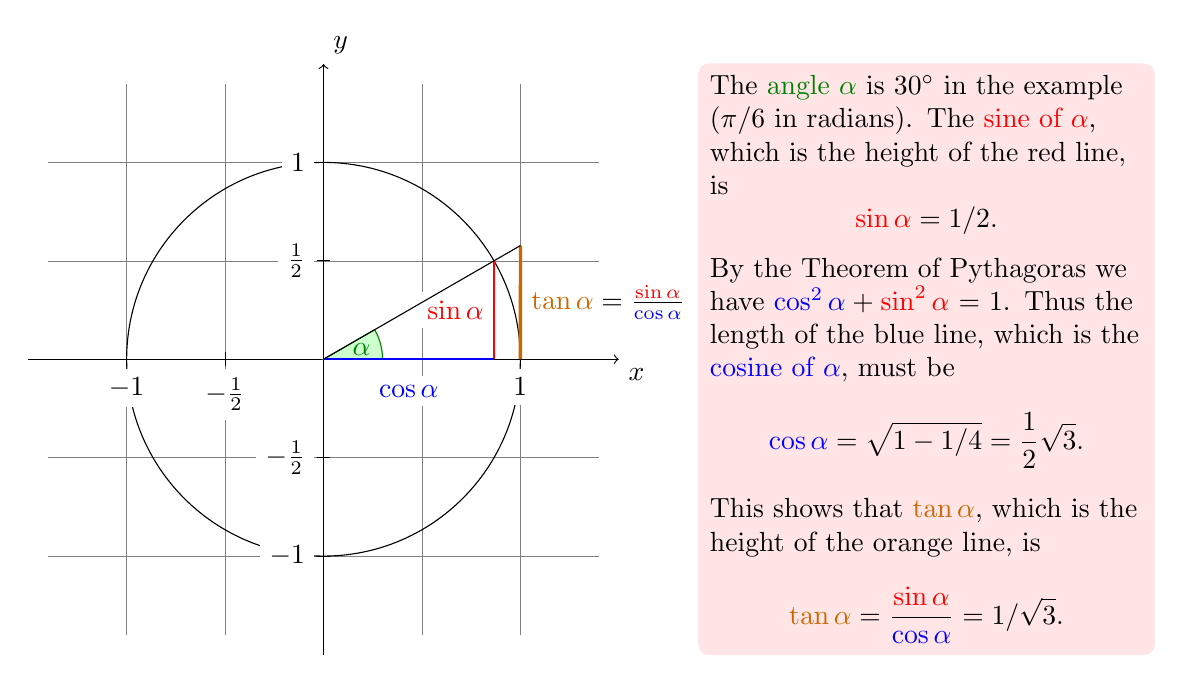
\begin{tikzpicture}
    [scale=2.5,
    % Styles
    axes/.style=,
    important line/.style={very thick},
    information text/.style={rounded corners,fill=red!10,inner sep=1ex}]
    
    % Colors
    \colorlet{anglecolor}{green!50!black}
    \colorlet{sincolor}{red}
    \colorlet{coscolor}{blue}
    \colorlet{tancolor}{orange!80!black}
    
    % Clip to isolate a part of the figure
    %\clip (-1,-1) rectangle (3,3);
    
    % Grid
    \draw [step=5mm, help lines, gray] (-1.4,-1.4) grid (1.4,1.4);
    
    % Circle
    \draw (0,0) circle [radius=1];
    
    % Draw coordinate system
    \draw[->] (-1.5,0) -- (1.5,0) node [anchor=north west] {$x$};
    \draw[->] (0,-1.5) -- (0,1.5) node [anchor=south west] {$y$};
    % Ticks and Labels
    \foreach \x/\xtext in {-1, -.5/-\frac{1}{2}, 1}
    \draw (\x,-1pt) -- (\x,1pt) node [below=2mm, fill=white] {$\xtext$};
    \foreach \y/\ytext in {-1, -.5/-\frac{1}{2}, .5/\frac{1}{2}, 1}
    \draw (-1pt,\y) -- (1pt,\y) node [left=2mm, fill=white] {$\ytext$};
    
    % Arc
    \filldraw[fill=green!20!white, draw=green!50!black] (0,0) -- (3mm,0) 
    arc [start angle = 0, end angle = 30, radius = 3mm] -- cycle;
    \draw (15:2mm) node[anglecolor] {$\alpha$};
    
    % Sin
    \draw[sincolor,thick]    (30:1) -- node[left,fill=white] {$\sin\alpha$} (30:1 |- 0,0);
    % Cos
    \draw[coscolor,thick]   (30:1) ++(0,-.5) -- node[below=2mm,fill=white] {$\cos\alpha$} (0,0);
    % Tan
    \path[name path=upward] (1,0) -- (1,1);
    \path[name path=sloped] (0,0) -- (30:1.5); 
    \draw[name intersections={of=upward and sloped, by = x}]
    [very thick, tancolor] (1,0) -- node[right] {$\tan\alpha\color{black}=\frac{{\color{sincolor}\sin\alpha}}{{\color{coscolor}\cos\alpha}}$} (x);
    \draw (0,0) -- (x);
    
    % Text Box
    \draw[xshift=1.9cm]
    node[right,text width = 5.5cm,information text] {
      The {\color{anglecolor} angle $\alpha$} is $30^\circ$ in the example ($\pi/6$ in radians). The {\color{sincolor}sine of $\alpha$}, which is the height of the red line, is
      \[{\color{sincolor} \sin \alpha} = 1/2.\] 
      By the Theorem of Pythagoras we have ${\color{coscolor}\cos^2\alpha}+{\color{sincolor}\sin^2\alpha}=1$. Thus the length of the blue line, which is the \textcolor{coscolor}{cosine of $\alpha$}, must be
      \[{\color{coscolor} \cos \alpha} = \sqrt{1-1/4}=\frac{1}{2}\sqrt{3}.\]
      This shows that ${\color{tancolor} \tan\alpha}$, which is the height of the orange line, is
      \[{\color{tancolor}\tan\alpha}=\frac{{\color{sincolor}\sin\alpha}}{{\color{coscolor}\cos\alpha}}=1/\sqrt{3}.\] 
      };
\end{tikzpicture}

%%%%%%%%%%%%%%%%%%%%%%%%%%%%%
%                           %
%          PETRI-NET        %
%                           %
%%%%%%%%%%%%%%%%%%%%%%%%%%%%%
\clearpage
\section{Tutorial: A Petri-Net for Hagen}

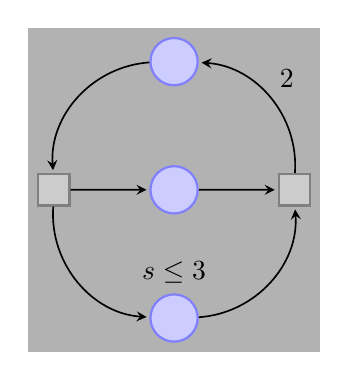
\begin{tikzpicture}
    [scale=3,
    bend angle=45,
    place/.style={circle,draw=blue!50,fill=blue!20,thick,
                  inner sep=0pt,minimum size=6mm},
    transition/.style={rectangle,draw=black!50,fill=black!20,thick,
                       inner sep=0pt,minimum size=4mm},
    pre/.style={<-,shorten <=1pt,>=stealth,semithick},
    post/.style={->,shorten >=1pt,>=stealth,semithick}]
                       
    \node[place] (waiting)  {};
    \node[place] (critical) [below=of waiting] {};
    \node[place] (semaphore)[below=of critical,
                             label=above:$s\leq3$] {};
                             
    \node[transition] (leave critical) [right=of critical] {}
        edge[pre]               (critical)
        edge[pre,bend left]     (semaphore)
        edge[post,bend right] node[auto,swap] {2}  (waiting);
    \node[transition] (enter critical) [left=of critical] {}
        edge[pre,bend left]     (waiting)
        edge[post]              (critical)
        edge[post,bend right]   (semaphore);
    
    \begin{scope}[on background layer]
        \node [fill=black!30,fit=(waiting) (semaphore) (leave critical) (enter critical)] {};
    \end{scope}
\end{tikzpicture}

%%%%%%%%%%%%%%%%%%%%%%%%%%%%%
%                           %
%           ANGLE           %
%                           %
%%%%%%%%%%%%%%%%%%%%%%%%%%%%%
\clearpage
\section{Angle}

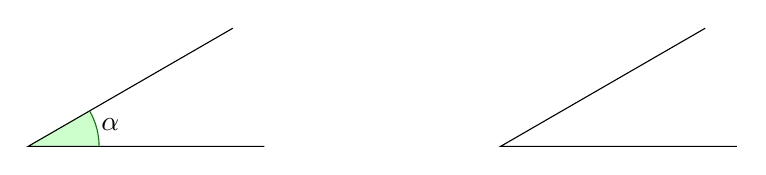
\begin{tikzpicture}[scale=3]
    \coordinate (A) at (30:1);
    \coordinate (B) at (0,0);
    \coordinate (C) at (1,0);
    
    \draw (A) -- (B) -- (C)
        pic [draw=green!50!black,fill=green!20,angle radius=9mm,angle eccentricity=1.2, "$\alpha$"] {angle = C--B--A};
        
    \draw (3,0) -- (2,0) -- +(30:1)
        pic [draw=green!50!black,fill=green!20,angle radius=9mm,angle eccentricity=1.2, "$\alpha$"] {};
\end{tikzpicture}

%%%%%%%%%%%%%%%%%%%%%%%%%%%%%
%                           %
%       BLOCH SPHERE        %
%                           %
%%%%%%%%%%%%%%%%%%%%%%%%%%%%%
\clearpage
\section{Bloch Sphere}

\begin{tikzpicture}
    [scale=3]
    
    % Circle
    \draw (0,0) circle [radius = 1cm];
    
    % Ellipse
    \draw[dashed] (0,0) ellipse [x radius = 1cm, y radius = .3 cm];
    
    % Draw Coordinate System
    \draw[->] (0,0) -- (225:.5) node[below left] {$x$};
    \draw[->] (0,0) -- (1,0) node[right] {$y$};
    \draw[->] (0,0) -- (0,1) node[above] {$z$};
    
    % Computational basis states
    \draw (0,-1) \node[below] {$|0\rangle$};
    \draw (0,1) \node[above] {$|1\rangle$};
    
    % Draw Bloch vector
    
\end{tikzpicture}

%%%%%%%%%%%%%%%%%%%%%%%%%%%%%
%                           %
%            JJ             %
%                           %
%%%%%%%%%%%%%%%%%%%%%%%%%%%%%
\clearpage
\section{Josephson Junction}
\newcommand{\wasd}{
    -- rectangle +(1,1);
    \draw (0,0) -- (1,1);
    \draw (1,0) -- (0,1);
}
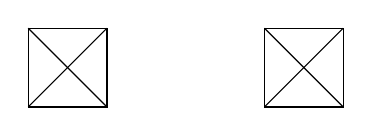
\begin{tikzpicture}
    % Josephson Junction
    \def\josephsonjunction at (#1,#2){
    \draw (#1,#2) rectangle ++(1,1);
    \draw (#1,#2) -- ++(1,1);
    \draw (#1,#2) +(1,0) -- +(0,1);
    }
    
    \josephsonjunction at (0,0);
    \josephsonjunction at (3,0);
\end{tikzpicture}

\end{document}